\documentclass[a4paper,12pt,preview]{report} %размер бумаги устанавливаем А4, шрифт 12пунктов
\usepackage[english,russian]{babel}%используем русский и английский языки с переносами 	
\usepackage[T2A]{fontenc}
\usepackage{changepage}
\usepackage{lipsum}
\usepackage{array}
\usepackage{indentfirst}
\usepackage[labelsep=period]{caption}
\usepackage{amsmath}
\usepackage{textcomp}
\usepackage[utf8]{inputenc}%включаем свою кодировку: koi8-r или utf8 в UNIX, cp1251 в Windows
\usepackage[english,russian]{babel}%используем русский и английский языки с переносами 	
\usepackage{amssymb,amsfonts,amsmath,mathtext,cite,enumerate,float} %подключаем нужные пакеты расширений
\usepackage{graphicx} %хотим вставлять в диплом рисунки?
\usepackage{ragged2e}
\usepackage{indentfirst}
\usepackage{titlesec}
\usepackage{listings}
\graphicspath{{images/}}%п\usepackage{trd}уть к рисункам



\makeatletter
\renewcommand{\@biblabel}[1]{#1.} % Заменяем библиографию с квадратных скобок на точку:
\makeatother

\usepackage{geometry} % Меняем поля страницы
\geometry{left=2cm}% левое поле
\geometry{right=1.5cm}% правое поле
\geometry{top=1cm}% верхнее поле
\geometry{bottom=2cm}% нижнее поле

\renewcommand{\theenumi}{\arabic{enumi}}% Меняем везде перечисления на цифра.цифра
\renewcommand{\labelenumi}{\arabic{enumi}}% Меняем везде перечисления на цифра.цифра
\renewcommand{\theenumii}{.\arabic{enumii}}% Меняем везде перечисления на цифра.цифра
\renewcommand{\labelenumii}{\arabic{enumi}.\arabic{enumii}.}% Меняем везде перечисления на цифра.цифра
\renewcommand{\theenumiii}{.\arabic{enumiii}}% Меняем везде перечисления на цифра.цифра
\renewcommand{\labelenumiii}{\arabic{enumi}.\arabic{enumii}.\arabic{enumiii}.}% Меняем везде перечисления на цифра.цифра

\newcommand{\doublerule}[1][.4pt]{%
	\noindent
	\makebox[0pt][l]{\rule[.7ex]{\linewidth}{#1}}%
	\rule[.3ex]{\linewidth}{#1}}


\titleformat{\chapter}[hang]
{\normalfont\huge\bfseries}{\thechapter.}{20pt}{}



\begin{document}
	
	\begin{center}
		Министерство образования и науки РФ \\
		Федеральное государственное автономное образовательное учреждение высшего профессионального образования <<НИТУ МИСиС>>\\
		Институт ИТАСУ\\
		Кафедра Инженерной кибернетики\\
	\end{center}
	
	
	\vfill
	
	\begin{center}
		\Large\textbf{Курсовая работа \\
			по курсу <<Специальные главы по базам данных>>}
	\end{center}
	
	\vfill
	
	\begin{FlushRight}
		Выполнил\\
		Студент группы \\
		БПМ-16-2 \\
		Фадеев А.Ю. \\
		[\baselineskip]
		Проверил: \\
		доц. Кожаринов А.С. \\
		[9\baselineskip]
	\end{FlushRight}
	
	
	\begin{center}
		Москва 2020
	\end{center}
	
	\thispagestyle{empty}
	\newpage
	
	\tableofcontents
	
	\newpage
	
	
	
	\chapter{Список основных используемых сокращений}
	
	БД - База Данных
	
	GUI - Graphical User Interface
	
	
	\chapter{Постановка задачи}
	
	\section{Описание предметной области}
	
	Разработанное приложение предназначено для предметной области "Секция спортивного программирования". В нем отражаются основные структуры секции ACM MISiS. 
	
	\section{Назначение разрабатываемой информационной системы}
	
	Разработанное приложение облегчает работу сотрудников секции, так как благодаря ему обеспечивается:
	
	\begin{enumerate}
		\item Быстрый и удобный доступ к данным.
		\item Интуитивно понятный алгоритм для добавления и удаления данных
		\item Распределение прав доступа к данным в зависимости от позиции сотружника
	\end{enumerate}
	
	\chapter{Использованные средства разработки и системные требования}
	
	\section{Описание языковых и инструментальных средств}
	
	База данных была спроектирована с помощью системы управления реляционными базами данных Microsoft SQL Server, в которой используется язык запросов Transact-SQL. Интерфейс приложения разработан в среде разработки Wing на языке Python3 с использованием библиотек PySimpleGUI, Pyodbc.
	
	\section{Системные требования для клиентского приложения и базы данных}

	Наличие Python3 и установленных PySimpleGUI, Pyodbc.
	
	
	\chapter{Модель данных}
	\section{ER-диаграмма}
	Диаграмма сущность-связь является удобным инструментом на этапе проектирования БД, так как наглядно отражает взаимосвязь сущностей и присущие им характеристики.
	
	При проведении исследования были выделены следующие сущности:
	\begin{itemize}
		\item Лицо
		\item Дивизион
		\item Занятие
		\item Помещение
		\item Команда
		\item Соревнования
		\item Сотрудники
	\end{itemize}
	
	На рисунке (Рисунок 1) можно увидеть диаграмму, получившуюся в ходе работы:
	
	\begin{center}
		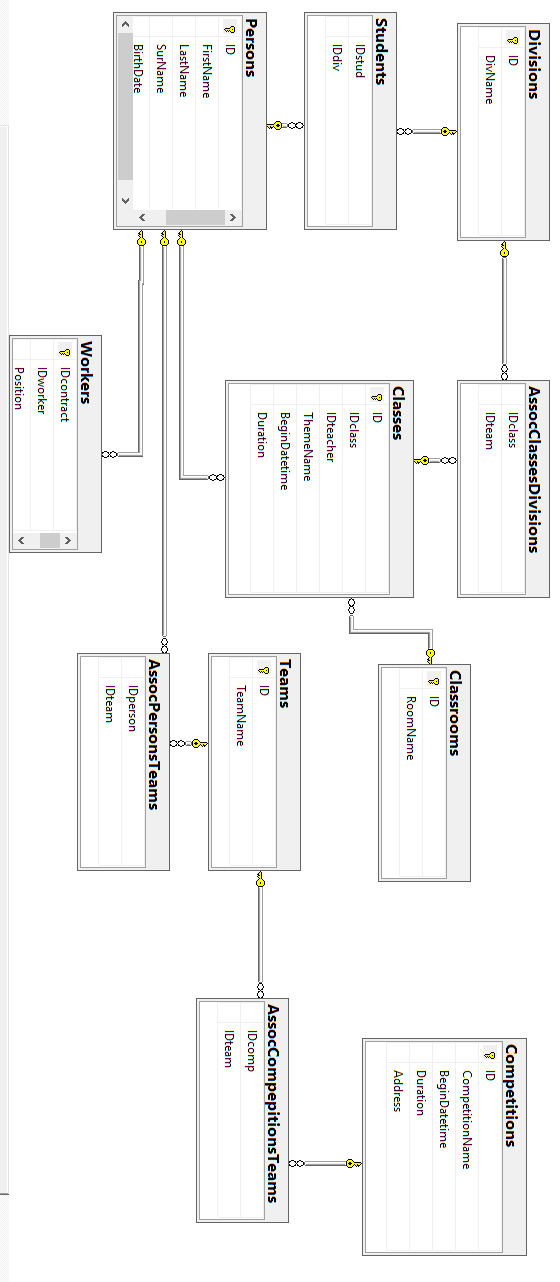
\includegraphics[scale=0.6]{ER.PNG}\\
		Рисунок 1. ER-диаграмма
	\end{center}
	
	\section{Особенности структуры модели}
	Рассмотрим более подробно сущности и соответствующие им атрибуты:
	\begin{itemize}
		\item Лицо" (Имя, Фамилия, Отчество, Дата рождения) -- хранит информацию о всех лицах, связанных с секцией.
		\item "Дивизион" (Название) -- хранит информацию о разделениях студентов на учебные группы.
		\item "Занятие" (ID помещения, ) -- хранит информацию о предстоящих или прошедших занятиях для дивизионов. 
		\item "Помещение" (Название) -- хранит информацию о всех учебных помещениях, в которых возможно проводить занятия.
		\item "Команда" (Название) -- хранит информацию о командах из 1-3 человек для участия в соревнованиях
		\item "Соревнование" (Название, Дата начала, Длительность, Адрес) -- хранит информацию о соревнованиях, в которых могут участвовать команды.
		\item "Сотрудники" (Должность, Номер контракта) -- хранит информацию о людях, работающих на секцию.
	\end{itemize}
	
	\begin{center}
		\begin{tabular}{ | m{5em} | m{5cm} | m{8cm} | } 
			\hline
			\textnumero & Название таблицы & Назначение \\ 	\hline \hline
			1 & Divisions & Хранит информацию о дивизионах \\ \hline
			2 & Students & Хранит информацию о студентах секции \\ \hline
			3 & Persons & Хранит информацию о всех людях, связанных с секцией \\ \hline
			4 & AssocClassesDivdisions & Хранит информацию о том, какие дивизионы на какие занятия записаны \\ \hline
			5 & Classes & Хранит информацию занятиях \\ \hline
			6 & Classrooms & Хранит информацию помещениях \\ \hline
			7 & Workers & Хранит информацию работниках \\ \hline
			8 & Teams & Хранит информацию о командах \\ \hline
			9 & AssocPersonsTeams & Хранит информацию о соответствии людей и команд \\ \hline
			10 & Competitions & Хранит информацию соревнованиях \\ \hline
			11 & AssocCompetitionsTeams & Хранит информацию соответствии соревнований и команд \\ \hline
		\end{tabular}
	\end{center}
	
	\chapter{Описание клиентского приложения}
	
	\section{назначение клиентсткого приложения и его функциональные особенности}
	
	Перечень реализованных в данной работе функций:
	\begin{itemize}
		\item Разделение ролей
		\item Ведение базы данных
		\item Отображение актуальной информации о участниках / командах / соревнованиях / занятиях / сотрудниках
		\item Вставка / удаление / изменение данных
	\end{itemize}
	
	\section{описание основных экранных форм}
	
	При начале работы с приложением открывается окно авторизации, в него пользователь вводит свои данные.
	
	\begin{center}
		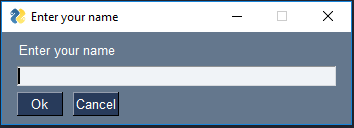
\includegraphics{autorization.PNG} \\
		Рисунок 2. окно авторизации
	\end{center}
	
	При нажатии кпопки "Ок" появляется следующее окно.
	
	
	\begin{center}
		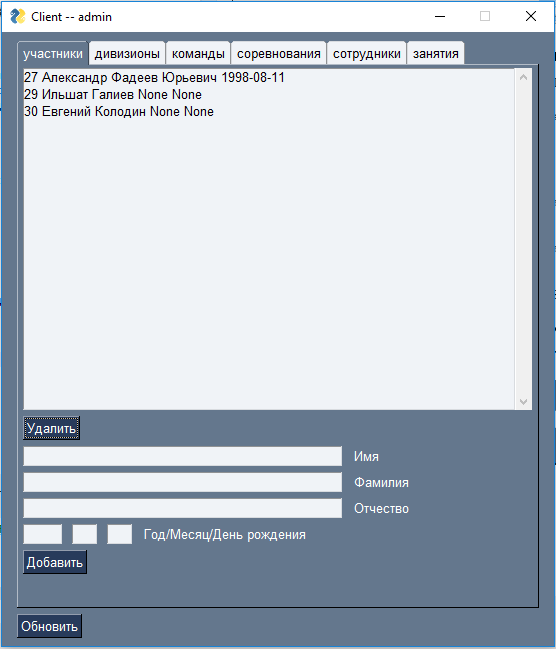
\includegraphics{members.PNG} \\
		Рисунок 3. Участники
	\end{center}
	
	Во вкладке "участники" возможно добавлять или удалять выбранного участника.
	

	
	\begin{center}
		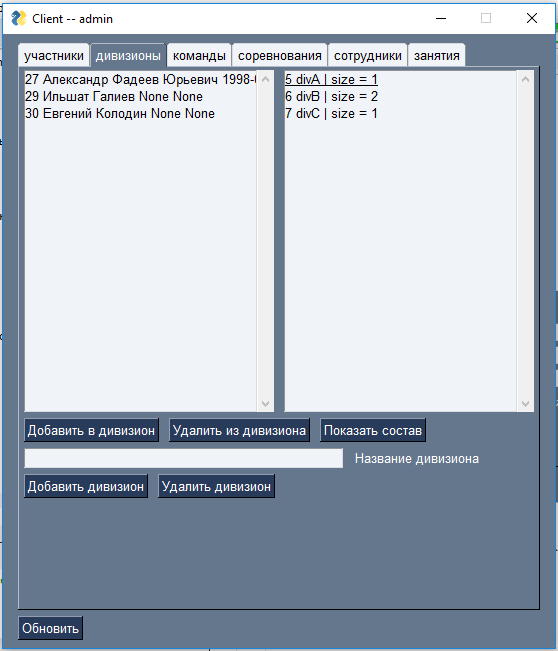
\includegraphics{divisions.PNG} \\
		Рисунок 4. Дивизионы
	\end{center}
	
	Во вкладке "дивизионы" возможно добавлять или удалять дивизион, можно добавить участника в дивизион или удалить из него, можно показать состав выбранного дивизиона или состав всех дивизионов.
	
	
	\begin{center}
		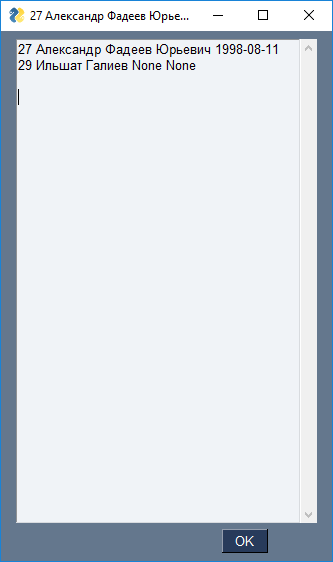
\includegraphics{onediv.PNG} \\
		Рисунок 5. Состав одного дивизиона
	\end{center}
	
	
	\begin{center}
		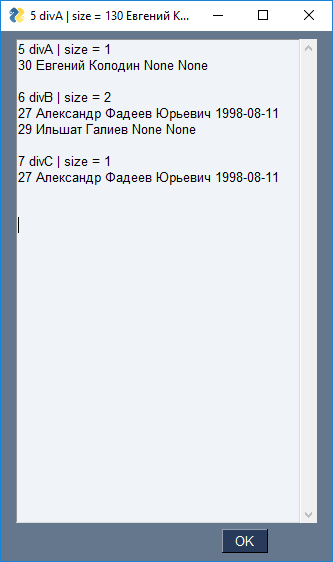
\includegraphics{alldivs.PNG} \\
		Рисунок 6. Состав всех дивизионов
	\end{center}
	
	
	
	\begin{center}
		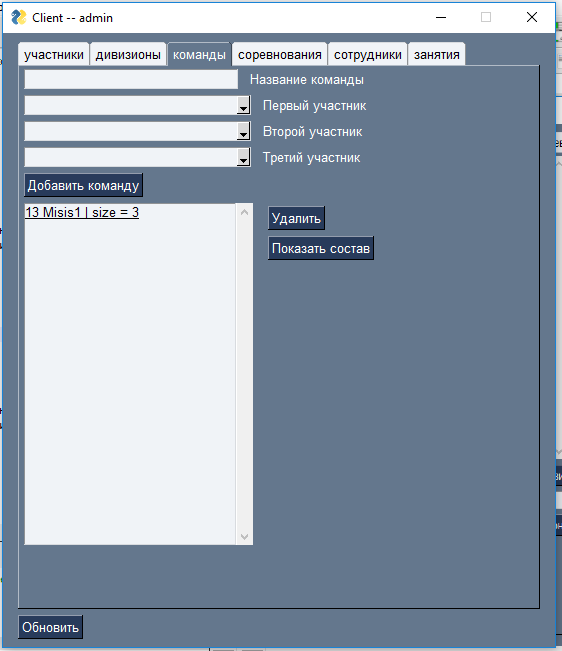
\includegraphics{teams.PNG} \\
		Рисунок 7. Команды
	\end{center}
	
	Во вкладке "команды" можно добавить команду из 1-3 участников, удалить выбранную команду, показать состав выбранной команды.
	
	
	
	
	
	\begin{center}
		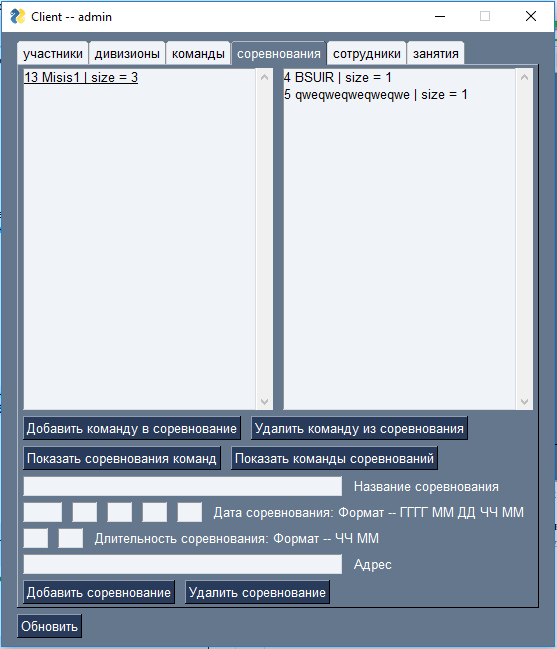
\includegraphics{competitions.PNG} \\
		Рисунок 8. Соревнования
	\end{center}
	
	Во вкладке "соревнования" можно добавить / удалить соревнование, добавить команду в соревнование или удалить из него, показать для одного или всех соревнований какие команды являются участниками, показать для одной или всех команд, в каких соревнованиях производится участие.
	
	
	
	
	
	
	\begin{center}
		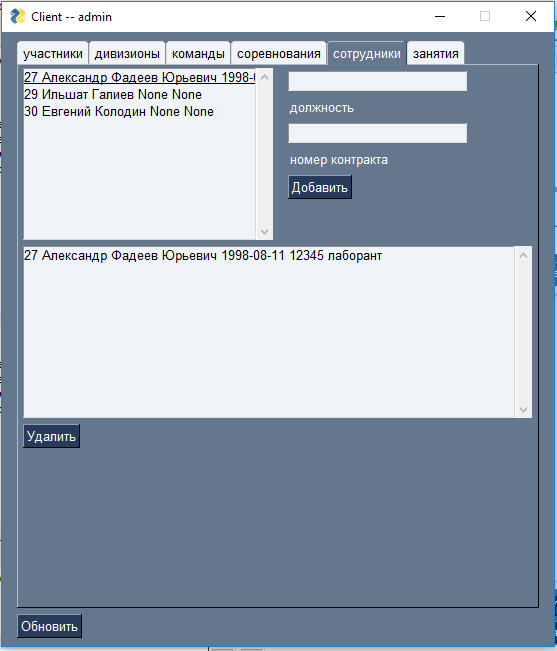
\includegraphics{workers.PNG} \\
		Рисунок 9. Сотрудники
	\end{center}
	
	Во вкладке "сотрудники" можно добавить / удалить сотрудника.
	
	
	
	
	\begin{center}
		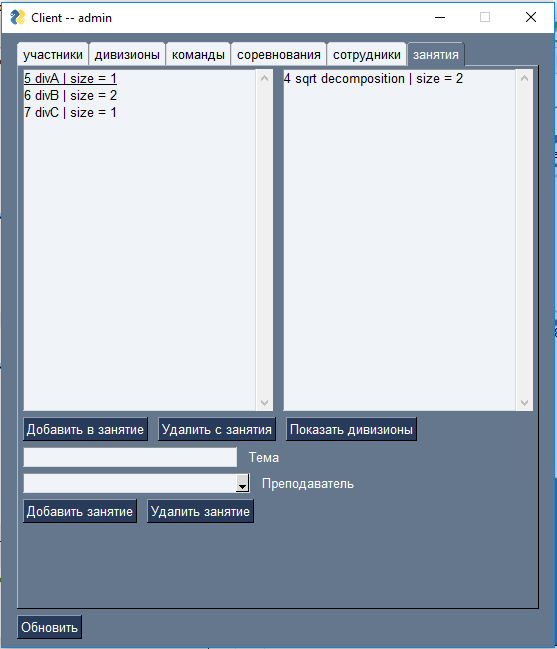
\includegraphics{classes.PNG} \\
		Рисунок 10. Занятия
	\end{center}
	
	Во вкладке "занятия" можно добавить / удалить занятия, добавить дивизион в занятие или удалить из него, показать для выбранного занятия какие дивизионы в нем участвуют.
	
	
	\chapter{Выводы}
	
	В рамках данной курсовой работы был выполнен системный анализ предметной области, в ходе которого были разработаны: структура базы данных, программная реализация БД, а также приложение Клиент-Сервер, которое упрощает работу с базой данных.
	
	
	\chapter{Список используемой литературы}
	
	\begin{enumerate}
		\item https://docs.microsoft.com/ru-ru/sql/sql-server/?view=sql-server-ver15
		\item https://github.com/mkleehammer/pyodbc/wiki
		\item https://pysimplegui.readthedocs.io/en/latest/
	\end{enumerate}
	
	\chapter{Приложения}
	
	\section{Скрипт для создания БД}
	\begin{verbatim}

USE [master]
GO
/****** Object:  Database [CompepativeProgrammingSection]    Script Date: 4/23/2020 3:10:51 AM ******/
CREATE DATABASE [CompepativeProgrammingSection]
 CONTAINMENT = NONE
 ON  PRIMARY 
( NAME = N'CompepativeProgrammingSection', FILENAME = N'C:\Program Files\Microsoft SQL Server\MSSQL14.SQLEXPRESS\MSSQL\DATA\CompepativeProgrammingSection.mdf' , SIZE = 8192KB , MAXSIZE = UNLIMITED, FILEGROWTH = 65536KB )
 LOG ON 
( NAME = N'CompepativeProgrammingSection_log', FILENAME = N'C:\Program Files\Microsoft SQL Server\MSSQL14.SQLEXPRESS\MSSQL\DATA\CompepativeProgrammingSection_log.ldf' , SIZE = 8192KB , MAXSIZE = 2048GB , FILEGROWTH = 65536KB )
GO
ALTER DATABASE [CompepativeProgrammingSection] SET COMPATIBILITY_LEVEL = 140
GO
IF (1 = FULLTEXTSERVICEPROPERTY('IsFullTextInstalled'))
begin
EXEC [CompepativeProgrammingSection].[dbo].[sp_fulltext_database] @action = 'enable'
end
GO
ALTER DATABASE [CompepativeProgrammingSection] SET ANSI_NULL_DEFAULT OFF 
GO
ALTER DATABASE [CompepativeProgrammingSection] SET ANSI_NULLS OFF 
GO
ALTER DATABASE [CompepativeProgrammingSection] SET ANSI_PADDING OFF 
GO
ALTER DATABASE [CompepativeProgrammingSection] SET ANSI_WARNINGS OFF 
GO
ALTER DATABASE [CompepativeProgrammingSection] SET ARITHABORT OFF 
GO
ALTER DATABASE [CompepativeProgrammingSection] SET AUTO_CLOSE OFF 
GO
ALTER DATABASE [CompepativeProgrammingSection] SET AUTO_SHRINK OFF 
GO
ALTER DATABASE [CompepativeProgrammingSection] SET AUTO_UPDATE_STATISTICS ON 
GO
ALTER DATABASE [CompepativeProgrammingSection] SET CURSOR_CLOSE_ON_COMMIT OFF 
GO
ALTER DATABASE [CompepativeProgrammingSection] SET CURSOR_DEFAULT  GLOBAL 
GO
ALTER DATABASE [CompepativeProgrammingSection] SET CONCAT_NULL_YIELDS_NULL OFF 
GO
ALTER DATABASE [CompepativeProgrammingSection] SET NUMERIC_ROUNDABORT OFF 
GO
ALTER DATABASE [CompepativeProgrammingSection] SET QUOTED_IDENTIFIER OFF 
GO
ALTER DATABASE [CompepativeProgrammingSection] SET RECURSIVE_TRIGGERS OFF 
GO
ALTER DATABASE [CompepativeProgrammingSection] SET  DISABLE_BROKER 
GO
ALTER DATABASE [CompepativeProgrammingSection] SET AUTO_UPDATE_STATISTICS_ASYNC OFF 
GO
ALTER DATABASE [CompepativeProgrammingSection] SET DATE_CORRELATION_OPTIMIZATION OFF 
GO
ALTER DATABASE [CompepativeProgrammingSection] SET TRUSTWORTHY OFF 
GO
ALTER DATABASE [CompepativeProgrammingSection] SET ALLOW_SNAPSHOT_ISOLATION OFF 
GO
ALTER DATABASE [CompepativeProgrammingSection] SET PARAMETERIZATION SIMPLE 
GO
ALTER DATABASE [CompepativeProgrammingSection] SET READ_COMMITTED_SNAPSHOT OFF 
GO
ALTER DATABASE [CompepativeProgrammingSection] SET HONOR_BROKER_PRIORITY OFF 
GO
ALTER DATABASE [CompepativeProgrammingSection] SET RECOVERY SIMPLE 
GO
ALTER DATABASE [CompepativeProgrammingSection] SET  MULTI_USER 
GO
ALTER DATABASE [CompepativeProgrammingSection] SET PAGE_VERIFY CHECKSUM  
GO
ALTER DATABASE [CompepativeProgrammingSection] SET DB_CHAINING OFF 
GO
ALTER DATABASE [CompepativeProgrammingSection] SET FILESTREAM( NON_TRANSACTED_ACCESS = OFF ) 
GO
ALTER DATABASE [CompepativeProgrammingSection] SET TARGET_RECOVERY_TIME = 60 SECONDS 
GO
ALTER DATABASE [CompepativeProgrammingSection] SET DELAYED_DURABILITY = DISABLED 
GO
ALTER DATABASE [CompepativeProgrammingSection] SET QUERY_STORE = OFF
GO
USE [CompepativeProgrammingSection]
GO
/****** Object:  Table [dbo].[AssocClassesDivisions]    Script Date: 4/23/2020 3:10:51 AM ******/
SET ANSI_NULLS ON
GO
SET QUOTED_IDENTIFIER ON
GO
CREATE TABLE [dbo].[AssocClassesDivisions](
	[IDclass] [int] NOT NULL,
	[IDteam] [int] NOT NULL
) ON [PRIMARY]
GO
/****** Object:  Table [dbo].[AssocCompepitionsTeams]    Script Date: 4/23/2020 3:10:51 AM ******/
SET ANSI_NULLS ON
GO
SET QUOTED_IDENTIFIER ON
GO
CREATE TABLE [dbo].[AssocCompepitionsTeams](
	[IDcomp] [int] NOT NULL,
	[IDteam] [int] NOT NULL
) ON [PRIMARY]
GO
/****** Object:  Table [dbo].[AssocPersonsTeams]    Script Date: 4/23/2020 3:10:51 AM ******/
SET ANSI_NULLS ON
GO
SET QUOTED_IDENTIFIER ON
GO
CREATE TABLE [dbo].[AssocPersonsTeams](
	[IDperson] [int] NOT NULL,
	[IDteam] [int] NOT NULL
) ON [PRIMARY]
GO
/****** Object:  Table [dbo].[Classes]    Script Date: 4/23/2020 3:10:51 AM ******/
SET ANSI_NULLS ON
GO
SET QUOTED_IDENTIFIER ON
GO
CREATE TABLE [dbo].[Classes](
	[ID] [int] IDENTITY(1,1) NOT NULL,
	[IDclass] [int] NULL,
	[IDteacher] [int] NULL,
	[ThemeName] [nvarchar](255) NULL,
	[BeginDatetime] [datetime] NULL,
	[Duration] [time](7) NULL,
PRIMARY KEY CLUSTERED 
(
	[ID] ASC
)WITH (PAD_INDEX = OFF, STATISTICS_NORECOMPUTE = OFF, IGNORE_DUP_KEY = OFF, ALLOW_ROW_LOCKS = ON, ALLOW_PAGE_LOCKS = ON) ON [PRIMARY]
) ON [PRIMARY]
GO
/****** Object:  Table [dbo].[Classrooms]    Script Date: 4/23/2020 3:10:51 AM ******/
SET ANSI_NULLS ON
GO
SET QUOTED_IDENTIFIER ON
GO
CREATE TABLE [dbo].[Classrooms](
	[ID] [int] IDENTITY(1,1) NOT NULL,
	[RoomName] [nvarchar](255) NOT NULL,
PRIMARY KEY CLUSTERED 
(
	[ID] ASC
)WITH (PAD_INDEX = OFF, STATISTICS_NORECOMPUTE = OFF, IGNORE_DUP_KEY = OFF, ALLOW_ROW_LOCKS = ON, ALLOW_PAGE_LOCKS = ON) ON [PRIMARY]
) ON [PRIMARY]
GO
/****** Object:  Table [dbo].[Competitions]    Script Date: 4/23/2020 3:10:51 AM ******/
SET ANSI_NULLS ON
GO
SET QUOTED_IDENTIFIER ON
GO
CREATE TABLE [dbo].[Competitions](
	[ID] [int] IDENTITY(1,1) NOT NULL,
	[CompetitionName] [nvarchar](255) NULL,
	[BeginDatetime] [datetime] NULL,
	[Duration] [time](7) NULL,
	[Address] [nvarchar](255) NULL,
PRIMARY KEY CLUSTERED 
(
	[ID] ASC
)WITH (PAD_INDEX = OFF, STATISTICS_NORECOMPUTE = OFF, IGNORE_DUP_KEY = OFF, ALLOW_ROW_LOCKS = ON, ALLOW_PAGE_LOCKS = ON) ON [PRIMARY]
) ON [PRIMARY]
GO
/****** Object:  Table [dbo].[Divisions]    Script Date: 4/23/2020 3:10:51 AM ******/
SET ANSI_NULLS ON
GO
SET QUOTED_IDENTIFIER ON
GO
CREATE TABLE [dbo].[Divisions](
	[ID] [int] IDENTITY(1,1) NOT NULL,
	[DivName] [nvarchar](255) NULL,
PRIMARY KEY CLUSTERED 
(
	[ID] ASC
)WITH (PAD_INDEX = OFF, STATISTICS_NORECOMPUTE = OFF, IGNORE_DUP_KEY = OFF, ALLOW_ROW_LOCKS = ON, ALLOW_PAGE_LOCKS = ON) ON [PRIMARY]
) ON [PRIMARY]
GO
/****** Object:  Table [dbo].[Persons]    Script Date: 4/23/2020 3:10:51 AM ******/
SET ANSI_NULLS ON
GO
SET QUOTED_IDENTIFIER ON
GO
CREATE TABLE [dbo].[Persons](
	[ID] [int] IDENTITY(1,1) NOT NULL,
	[FirstName] [nvarchar](255) NOT NULL,
	[LastName] [nvarchar](255) NOT NULL,
	[SurName] [nvarchar](255) NULL,
	[BirthDate] [date] NULL,
PRIMARY KEY CLUSTERED 
(
	[ID] ASC
)WITH (PAD_INDEX = OFF, STATISTICS_NORECOMPUTE = OFF, IGNORE_DUP_KEY = OFF, ALLOW_ROW_LOCKS = ON, ALLOW_PAGE_LOCKS = ON) ON [PRIMARY]
) ON [PRIMARY]
GO
/****** Object:  Table [dbo].[Students]    Script Date: 4/23/2020 3:10:51 AM ******/
SET ANSI_NULLS ON
GO
SET QUOTED_IDENTIFIER ON
GO
CREATE TABLE [dbo].[Students](
	[IDstud] [int] NOT NULL,
	[IDdiv] [int] NOT NULL
) ON [PRIMARY]
GO
/****** Object:  Table [dbo].[Teams]    Script Date: 4/23/2020 3:10:51 AM ******/
SET ANSI_NULLS ON
GO
SET QUOTED_IDENTIFIER ON
GO
CREATE TABLE [dbo].[Teams](
	[ID] [int] IDENTITY(1,1) NOT NULL,
	[TeamName] [nvarchar](255) NOT NULL,
PRIMARY KEY CLUSTERED 
(
	[ID] ASC
)WITH (PAD_INDEX = OFF, STATISTICS_NORECOMPUTE = OFF, IGNORE_DUP_KEY = OFF, ALLOW_ROW_LOCKS = ON, ALLOW_PAGE_LOCKS = ON) ON [PRIMARY]
) ON [PRIMARY]
GO
/****** Object:  Table [dbo].[Workers]    Script Date: 4/23/2020 3:10:51 AM ******/
SET ANSI_NULLS ON
GO
SET QUOTED_IDENTIFIER ON
GO
CREATE TABLE [dbo].[Workers](
	[IDcontract] [int] NOT NULL,
	[IDworker] [int] NOT NULL,
	[Position] [nvarchar](255) NULL,
PRIMARY KEY CLUSTERED 
(
	[IDcontract] ASC
)WITH (PAD_INDEX = OFF, STATISTICS_NORECOMPUTE = OFF, IGNORE_DUP_KEY = OFF, ALLOW_ROW_LOCKS = ON, ALLOW_PAGE_LOCKS = ON) ON [PRIMARY]
) ON [PRIMARY]
GO
ALTER TABLE [dbo].[AssocClassesDivisions]  WITH CHECK ADD FOREIGN KEY([IDclass])
REFERENCES [dbo].[Classes] ([ID])
ON DELETE CASCADE
GO
ALTER TABLE [dbo].[AssocClassesDivisions]  WITH CHECK ADD FOREIGN KEY([IDteam])
REFERENCES [dbo].[Divisions] ([ID])
ON DELETE CASCADE
GO
ALTER TABLE [dbo].[AssocCompepitionsTeams]  WITH CHECK ADD FOREIGN KEY([IDcomp])
REFERENCES [dbo].[Competitions] ([ID])
ON DELETE CASCADE
GO
ALTER TABLE [dbo].[AssocCompepitionsTeams]  WITH CHECK ADD FOREIGN KEY([IDteam])
REFERENCES [dbo].[Teams] ([ID])
ON DELETE CASCADE
GO
ALTER TABLE [dbo].[AssocPersonsTeams]  WITH CHECK ADD FOREIGN KEY([IDperson])
REFERENCES [dbo].[Persons] ([ID])
ON DELETE CASCADE
GO
ALTER TABLE [dbo].[AssocPersonsTeams]  WITH CHECK ADD FOREIGN KEY([IDteam])
REFERENCES [dbo].[Teams] ([ID])
ON DELETE CASCADE
GO
ALTER TABLE [dbo].[Classes]  WITH CHECK ADD FOREIGN KEY([IDclass])
REFERENCES [dbo].[Classrooms] ([ID])
ON DELETE CASCADE
GO
ALTER TABLE [dbo].[Classes]  WITH CHECK ADD FOREIGN KEY([IDteacher])
REFERENCES [dbo].[Persons] ([ID])
ON DELETE CASCADE
GO
ALTER TABLE [dbo].[Students]  WITH CHECK ADD FOREIGN KEY([IDdiv])
REFERENCES [dbo].[Divisions] ([ID])
ON DELETE CASCADE
GO
ALTER TABLE [dbo].[Students]  WITH CHECK ADD FOREIGN KEY([IDstud])
REFERENCES [dbo].[Persons] ([ID])
ON DELETE CASCADE
GO
ALTER TABLE [dbo].[Workers]  WITH CHECK ADD FOREIGN KEY([IDworker])
REFERENCES [dbo].[Persons] ([ID])
ON DELETE CASCADE
GO
USE [master]
GO
ALTER DATABASE [CompepativeProgrammingSection] SET  READ_WRITE 
GO


	\end{verbatim}
	
	\section{Скрипт для приложения}
	
\begin{verbatim}
import PySimpleGUI as sg
import pyodbc 
server_name = 'DESKTOP-3J853GC\SQLEXPRESS'
db_name = 'CompepativeProgrammingSection'
conn = pyodbc.connect('Driver={SQL Server};'
                      'Server='+server_name+';'
                      'Database='+db_name+';'
                      'Trusted_Connection=yes;')
cursor = conn.cursor()

current_user = sg.popup_get_text('Enter your name')
fl = False
if current_user == 'admin':
    fl = True

'=============== MEMBERS ==================='
members = {}
tab_members = [];
tab_members.append([sg.Listbox([], key='allmembers', size=(70, 20))])
if fl:
    tab_members.append([sg.Button(u'Удалить', key='member_delete')])
    tab_members.append([sg.InputText(key='firstname_add_members'), sg.Text(u'Имя')])
    tab_members.append([sg.InputText(key='secondname_add_members'), sg.Text(u'Фамилия')])
    tab_members.append([sg.InputText(key='surname_add_members'), sg.Text(u'Отчество')])
    tab_members.append([sg.InputText(key='year_add_members', size=(5, 1)), sg.InputText(key='month_add_members', size=(3, 1)), sg.InputText(key='day_add_members', size=(3, 1)), sg.Text(u'Год/Месяц/День рождения')])
    tab_members.append([sg.Button(u'Добавить', key='member_add')])

def update_members():
    global cursor
    cursor.execute('SELECT * FROM '+db_name+'.dbo.'+'Persons')
    global members
    members = {}
    list_members = []
    for row in cursor:
        curstr = ''
        for i in row:
            curstr += str(i) + ' '
        members[curstr] = row[0]
        list_members.append(curstr)
    window['allmembers'].update(list_members)
    window['allmembers_division'].update(list_members)
    if fl:
        window['listbox_workers_members'].update(list_members)
        window['first_team_member'].update(values=['']+list_members)
        window['second_team_member'].update(values=['']+list_members)
        window['third_team_member'].update(values=['']+list_members)
        window['combo_classes_member'].update(values=['']+list_members)
    
    
def delete_member():
    global values
    global members
    global cursor
    if (event != 'member_delete'):
        return;
    if (values['allmembers'] == []):
        return;
    ind = members[values['allmembers'][0]]
    cursor.execute('DELETE FROM '+db_name+'.dbo.'+'Persons WHERE ID =' + str(ind))
    conn.commit()
    #print(ind)

def add_member():
    global values
    global members
    global cursor
    if (event != 'member_add'):
        return;
    to_insert = '('
    if (values['firstname_add_members'] != ''):
        to_insert += 'N\'' + values['firstname_add_members'] + '\', '
    else:
        to_insert += 'NULL, '
        
    if (values['secondname_add_members'] != ''):
        to_insert += 'N\'' + values['secondname_add_members'] + '\', '
    else:
        to_insert += 'NULL, '
        
    if (values['surname_add_members'] != ''):
        to_insert += 'N\'' + values['surname_add_members'] + '\', '
    else:
        to_insert += 'NULL, '
    
    if (values['year_add_members'] != '' and values['month_add_members'] != '' and values['day_add_members'] != ''):
        date = '\'' + values['year_add_members']+'-'+values['month_add_members']+'-'+values['day_add_members'] + '\''
    else:
        date = 'NULL'
    
    to_insert += date
    to_insert += ')'
    #print(to_insert)
    query = u'INSERT INTO '+db_name+'.dbo.'+'Persons (FirstName, LastName, SurName, BirthDate) VALUES ' + to_insert + ';'
    #print(query)
    try:
        cursor.execute(query)
        conn.commit()
    except:
        sg.Popup('Что-то пошло не так')
    
    
    
        
'=============== DIVISIONS ==================='
divisions = {}
tab_divisions = [];
tab_divisions.append([sg.Listbox([], key='allmembers_division', size=(33, 20)), sg.Listbox([], key='alldivision', size=(33, 20))])
if fl:
    tab_divisions.append([sg.Button(u'Добавить в дивизион', key='button_div_add'), sg.Button(u'Удалить из дивизиона', key='button_div_remove'), sg.Button(u'Показать состав', key='show_all_in_div')])
    tab_divisions.append([sg.InputText(key='add_division'), sg.Text(u'Название дивизиона')])
    tab_divisions.append([sg.Button(u'Добавить дивизион', key='division_add'), sg.Button(u'Удалить дивизион', key='division_remove')])
else:
    tab_divisions.append([sg.Button(u'Показать состав', key='show_all_in_div')])
    
def update_divisions():
    global cursor
    cursor.execute('SELECT * FROM '+db_name+'.dbo.'+'Divisions')
    global divisions
    data = [row for row in cursor]
    divisions = {}
    list_divisions = []
    for row in data:
        cursor.execute('SELECT * FROM '+db_name+'.dbo.'+'Students WHERE IDdiv = ' + str(row[0]))
        curstr = ''
        for i in row:
            curstr += str(i) + ' '
        num = 0
        ddata = [row for row in cursor]
        curstr += '| size = '+str(len(ddata))
        divisions[curstr] = row[0]
        list_divisions.append(curstr)
    window['alldivision'].update(list_divisions)
    window['listbox_classes_divisions'].update(list_divisions)
    #print(list_divisions)
    
def add_to_division():
    global event
    global values
    global members
    if (event != 'button_div_add'):
        return;
    if (values['allmembers_division'] == []):
        return;
    if (values['alldivision'] == []):
        return;
    indmem = str(members[values['allmembers_division'][0]])
    inddiv = str(divisions[values['alldivision'][0]])

    to_insert = '(\'' + indmem + '\', \'' + inddiv + '\')'
    query = u'INSERT INTO '+db_name+'.dbo.'+'Students (IDstud, IDdiv) VALUES ' + to_insert + ';'
    try:
        cursor.execute('DELETE FROM '+db_name+'.dbo.'+'Students WHERE IDstud = ' + indmem + ' AND ' + 'IDdiv = ' + inddiv)
        #print(query)
        cursor.execute(query)
        conn.commit()        
    except:
        sg.Popup('Что-то пошло не так')
        
    
    
def remove_from_division():
    global event
    global values
    global members
    if (event != 'button_div_remove'):
        return;
    if (values['allmembers_division'] == []):
        return;
    if (values['alldivision'] == []):
        return;
    indmem = str(members[values['allmembers_division'][0]])
    inddiv = str(divisions[values['alldivision'][0]])
    cursor.execute('DELETE FROM '+db_name+'.dbo.'+'Students WHERE IDstud = ' + indmem + ' AND ' + 'IDdiv = ' + inddiv)
    conn.commit()

def show_in_div():
    global event
    global values
    if (event != 'show_all_in_div'):
        return;
    if (values['alldivision'] == []):
        return;
    inddiv = str(divisions[values['alldivision'][0]])
    query = 'SELECT P.* FROM Persons P INNER JOIN Students S ON P.ID = S.Idstud WHERE IDdiv = ' + inddiv + ' ORDER BY ID'
    cursor.execute(query)
    text = ''
    for row in cursor:
        for i in row:
            text += str(i) + ' '
        text += '\n'
    sg.popup_scrolled(text, size=(40, 30))

def show_all_divs():
    global event
    global values
    if (event != 'show_all_in_div'):
        return;
    if (values['alldivision'] != []):
        return;
    
    text = ''
    for div in divisions:
        inddiv = str(divisions[div])
        query = 'SELECT P.* FROM Persons P INNER JOIN Students S ON P.ID = S.Idstud WHERE IDdiv = ' + inddiv + ' ORDER BY ID'
        cursor.execute(query)
        text += div + '\n'
        for row in cursor:
            for i in row:
                text += str(i) + ' '
            text += '\n'
        text += '\n'
    sg.popup_scrolled(text, size=(40, 30))
    

def add_div():
    global values
    global members
    global cursor
    if (event != 'division_add'):
        return;
    to_insert = '('
    if (values['add_division'] != ''):
        to_insert += 'N\'' + values['add_division'] + '\' '
    else:
        to_insert += 'NULL '
    
    to_insert += ')'
    #print(to_insert)
    query = u'INSERT INTO '+db_name+'.dbo.'+'Divisions (DivName) VALUES ' + to_insert + ';'
    #print(query)
    try:
        cursor.execute(query)
        conn.commit()
    except:
        sg.Popup('Что-то пошло не так')    

def remove_div():
    global values
    global members
    global cursor
    if (event != 'division_remove'):
        return;
    if (values['alldivision'] == []):
        return;
    ind = divisions[values['alldivision'][0]]
    cursor.execute('DELETE FROM '+db_name+'.dbo.'+'Divisions WHERE ID =' + str(ind))
    conn.commit()
    #print(ind)

    
'=============== TEAMS ==================='
teams = {}
tab_teams = [];
if fl:
    tab_teams.append([sg.InputText(key='inputtext_team_name', size=(30, 1)), sg.Text('Название команды')])
    tab_teams.append([sg.Combo([], key='first_team_member', size=(30, 20)), sg.Text('Первый участник')])
    tab_teams.append([sg.Combo([], key='second_team_member', size=(30, 20)), sg.Text('Второй участник')])
    tab_teams.append([sg.Combo([], key='third_team_member', size=(30, 20)), sg.Text('Третий участник')])
    tab_teams.append([sg.Button('Добавить команду', key='button_add_team')])
    tab_teams.append([sg.Listbox([], key='listbox_teams', size=(30, 20)), sg.Column([[sg.Button('Удалить', key='button_delete_team')], [sg.Button('Показать состав', key='button_show_team')]])])
else:
    tab_teams.append([sg.Listbox([], key='listbox_teams', size=(30, 20)), sg.Column([[sg.Button('Показать состав', key='button_show_team')]])])


def update_teams():
    global cursor
    cursor.execute('SELECT * FROM '+db_name+'.dbo.Teams')
    global teams
    data = [row for row in cursor]
    teams = {}
    list_teams = []
    for row in data:
        cursor.execute('SELECT * FROM '+db_name+'.dbo.AssocPersonsTeams WHERE IDteam = ' + str(row[0]))
        curstr = ''
        for i in row:
            curstr += str(i) + ' '
        num = 0
        ddata = [row for row in cursor]
        curstr += '| size = '+str(len(ddata))
        teams[curstr] = row[0]
        list_teams.append(curstr)
    window['listbox_teams'].update(list_teams)
    window['listbox_teams_competitions'].update(list_teams)
    #print(list_teams)

def remove_team():
    global values
    global members
    global cursor
    if (event != 'button_delete_team'):
        return;
    if (values['listbox_teams'] == []):
        return;
    ind = teams[values['listbox_teams'][0]]
    cursor.execute('DELETE FROM '+db_name+'.dbo.Teams WHERE ID =' + str(ind))
    conn.commit()
    #print(ind)


def add_team():
    global event
    global values
    global cursor
    global conn
    global members
    if event != 'button_add_team':
        return
    if values['first_team_member'] == '' and values['second_team_member'] == '' and values['third_team_member'] == '':
        return
    if values['inputtext_team_name'] == '':
        return
    query = 'INSERT INTO '+db_name+'.dbo.Teams (TeamName) VALUES (N\''+values['inputtext_team_name']+'\')'
    cursor.execute(query)
    #print(query)
    query = 'SELECT ID FROM '+db_name+'.dbo.Teams WHERE TeamName = '+'N\''+values['inputtext_team_name']+'\''
    cursor.execute(query)
    #print(query)    
    indname = '-1'
    for row in cursor:
        indname = str(row[0])
    #print(indname)
    vals = [values['first_team_member'], values['second_team_member'], values['third_team_member']]
    #print(vals)
    for v in vals:
        if v != '':
            indpers = str(members[v])
            
            query = 'DELETE FROM '+db_name+'.dbo.AssocPersonsTeams WHERE IDperson = '+indpers+' AND IDteam = '+indname
            #print(query)
            cursor.execute(query)
            
            query = 'INSERT INTO '+db_name+'.dbo.AssocPersonsTeams (IDperson, IDteam) VALUES'+'('+indpers+', '+indname+')'
            #print(query)
            cursor.execute(query)
    conn.commit()    

def show_in_team():
    global event
    global values
    if (event != 'button_show_team'):
        return;
    if (values['listbox_teams'] == []):
        return;
    indteam = str(teams[values['listbox_teams'][0]])
    query = 'SELECT P.* FROM Persons P INNER JOIN AssocPersonsTeams A ON P.ID = A.IDperson WHERE IDteam = ' + indteam + ' ORDER BY ID'
    cursor.execute(query)
    text = ''
    for row in cursor:
        for i in row:
            text += str(i) + ' '
        text += '\n'
    sg.popup_scrolled(text, size=(40, 30))

def show_all_teams():
    global event
    global values
    if (event != 'button_show_team'):
        return;
    if (values['alldivision'] != []):
        return;
    
    text = ''
    for team in teams:
        indteam = str(teams[team])
        query = 'SELECT P.* FROM Persons P INNER JOIN AssocPersonsTeams A ON P.ID = A.IDperson WHERE IDteam = ' + indteam + ' ORDER BY ID'
        cursor.execute(query)
        text += team + '\n'
        for row in cursor:
            for i in row:
                text += str(i) + ' '
            text += '\n'
        text += '\n'
    sg.popup_scrolled(text, size=(40, 30))

    
'=============== COMPETITIONS ================='
competitions = {}
tab_competitions = []
tab_competitions.append([sg.Listbox([], key='listbox_teams_competitions', size=(33, 20)), sg.Listbox([], key='listbox_competitions', size=(33, 20))])
tab_competitions.append([sg.Button('Добавить команду в соревнование', key='button_add_team_to_competition'), sg.Button('Удалить команду из соревнования', key='button_delete_team_from_competition')])
tab_competitions.append([sg.Button('Показать соревнования команд', key='button_show_competitions'), sg.Button('Показать команды соревнований', key='button_show_teams')])
tab_competitions.append([sg.InputText(key='inputtext_competition_name'), sg.Text('Название соревнования')])
competition_date = []
competition_date.append(sg.InputText(key='inputtext_competition_year', size = (5, 1)))
competition_date.append(sg.InputText(key='inputtext_competition_month', size = (3, 1)))
competition_date.append(sg.InputText(key='inputtext_competition_day', size = (3, 1)))
competition_date.append(sg.InputText(key='inputtext_competition_hour', size = (3, 1)))
competition_date.append(sg.InputText(key='inputtext_competition_minute', size = (3, 1)))
competition_date.append(sg.Text('Дата соревнования: Формат -- ГГГГ ММ ДД ЧЧ ММ'))
tab_competitions.append(competition_date)
competition_duration = []
competition_duration.append(sg.InputText(key='inputtext_competition_duration_hour', size = (3, 1)))
competition_duration.append(sg.InputText(key='inputtext_competition_duration_minute', size = (3, 1)))
competition_duration.append(sg.Text('Длительность соревнования: Формат -- ЧЧ ММ'))
tab_competitions.append(competition_duration)
tab_competitions.append([sg.InputText(key='inputtext_competition_address'), sg.Text('Адрес')])
tab_competitions.append([sg.Button('Добавить соревнование', key='button_add_competition'), sg.Button('Удалить соревнование', key='button_remove_competition')])

if not fl:
    tab_competitions = []
    tab_competitions.append([sg.Listbox([], key='listbox_teams_competitions', size=(33, 20)), sg.Listbox([], key='listbox_competitions', size=(33, 20))])
    tab_competitions.append([sg.Button('Показать соревнования команд', key='button_show_competitions'), sg.Button('Показать команды соревнований', key='button_show_teams')])



def update_competitions():
    global cursor
    cursor.execute('SELECT ID, CompetitionName FROM '+db_name+'.dbo.Competitions')
    global competitions
    data = [row for row in cursor]
    competitions = {}
    list_competitions = []
    for row in data:
        cursor.execute('SELECT * FROM '+db_name+'.dbo.AssocCompepitionsTeams WHERE IDcomp = ' + str(row[0]))
        curstr = ''
        for i in row:
            curstr += str(i) + ' '
        num = 0
        ddata = [row for row in cursor]
        curstr += '| size = '+str(len(ddata))
        competitions[curstr] = row[0]
        list_competitions.append(curstr)
    window['listbox_competitions'].update(list_competitions)
    #print(list_competitions)

def add_to_competition():
    global event
    global values
    global teams
    global competitions
    if (event != 'button_add_team_to_competition'):
        return;
    if (values['listbox_competitions'] == []):
        return;
    if (values['listbox_teams_competitions'] == []):
        return;
    indcomp = str(competitions[values['listbox_competitions'][0]])
    indteam = str(teams[values['listbox_teams_competitions'][0]])

    to_insert = '(' + indcomp + ', ' + indteam + ')'
    #print(to_insert)
    query = u'INSERT INTO '+db_name+'.dbo.AssocCompepitionsTeams (IDcomp, IDteam) VALUES ' + to_insert + ';'
    try:
        cursor.execute('DELETE FROM '+db_name+'.dbo.AssocCompepitionsTeams WHERE IDcomp = ' + indcomp + ' AND ' + 'IDteam = ' + indteam)
        #print(query)
        cursor.execute(query)
        conn.commit()        
    except:
        sg.Popup('Что-то пошло не так')
        
    
    
def remove_from_competition():
    global event
    global values
    global teams
    global competitions
    if (event != 'button_delete_team_from_competition'):
        return;
    if (values['listbox_competitions'] == []):
        return;
    if (values['listbox_teams_competitions'] == []):
        return;
    indcomp = str(competitions[values['listbox_competitions'][0]])
    indteam = str(teams[values['listbox_teams_competitions'][0]])
    cursor.execute('DELETE FROM '+db_name+'.dbo.AssocCompepitionsTeams WHERE IDcomp = ' + indcomp + ' AND ' + 'IDteam = ' + indteam)
    conn.commit()
    
def add_competition():
    if event != 'button_add_competition':
        return
    if values['inputtext_competition_name'] == '':
        return
    to_insert = '(\'' + values['inputtext_competition_name'] + '\', '
    
    good = True
    if values['inputtext_competition_year'] == '':
        good = False
    if values['inputtext_competition_month'] == '':
        good = False
    if values['inputtext_competition_day'] == '':
        good = False
    if values['inputtext_competition_hour'] == '':
        good = False
    if values['inputtext_competition_minute'] == '':
        good = False
    
    if good == True:
        to_insert += '\''
        to_insert += values['inputtext_competition_year'] + '-'
        to_insert += values['inputtext_competition_month'] + '-'
        to_insert += values['inputtext_competition_day'] + 'T'
        to_insert += values['inputtext_competition_hour'] + ':'
        to_insert += values['inputtext_competition_minute'] + ':00.000'
        to_insert += '\', '
    else:
        to_insert += 'NULL, '
    
    
    good = True
    if values['inputtext_competition_duration_hour'] == '':
        good = False
    if values['inputtext_competition_duration_minute'] == '':
        good = False
    
    if good == True:
        to_insert += '\''
        to_insert += values['inputtext_competition_duration_hour'] + ':'
        to_insert += values['inputtext_competition_duration_minute'] + ':00.0000000'
        to_insert += '\', '
    else:
        to_insert += 'NULL, '
    
    if values['inputtext_competition_address'] != '':
        to_insert += '\'' + values['inputtext_competition_address'] + '\''
    else:
        to_insert += 'NULL'
    to_insert += ')'
    
    query = 'INSERT INTO '+db_name+'.dbo.Competitions (CompetitionName, BeginDatetime, Duration, Address) VALUES '+to_insert
    #print(query)
    cursor.execute(query)
    conn.commit()
    
def remove_competition():
    global values
    global competitions
    global cursor
    if (event != 'button_remove_competition'):
        return;
    if (values['listbox_competitions'] == []):
        return;
    ind = competitions[values['listbox_competitions'][0]]
    cursor.execute('DELETE FROM '+db_name+'.dbo.Competitions WHERE ID =' + str(ind))
    conn.commit()

def show_competitions_for_team():
    global event
    global values
    if (event != 'button_show_competitions'):
        return;
    if (values['listbox_teams_competitions'] == []):
        return;
    indteam = str(teams[values['listbox_teams_competitions'][0]])
    query = 'SELECT C.* FROM Competitions C INNER JOIN AssocCompepitionsTeams A ON C.ID = A.IDcomp WHERE IDteam = ' + indteam + ' ORDER BY ID'
    cursor.execute(query)
    text = ''
    for row in cursor:
        for i in row:
            text += str(i) + ' '
        text += '\n'
    sg.popup_scrolled(text, size=(70, 30))


def show_competitions_for_all_teams():
    global event
    global values
    if (event != 'button_show_competitions'):
        return;
    if (values['listbox_teams_competitions'] != []):
        return;
    
    text = ''
    for team in teams:
        indteam = str(teams[team])
        query = 'SELECT C.* FROM Competitions C INNER JOIN AssocCompepitionsTeams A ON C.ID = A.IDcomp WHERE IDteam = ' + indteam + ' ORDER BY ID'        
        cursor.execute(query)
        text += team + '\n'
        for row in cursor:
            for i in row:
                text += str(i) + ' '
            text += '\n'
        text += '\n'
    sg.popup_scrolled(text, size=(70, 30))

def show_teams_for_competition():
    global event
    global values
    if (event != 'button_show_teams'):
        return;
    if (values['listbox_competitions'] == []):
        return;
    indcomp = str(competitions[values['listbox_competitions'][0]])
    query = 'SELECT T.* FROM Teams T INNER JOIN AssocCompepitionsTeams A ON T.ID = A.IDteam WHERE IDcomp = ' + indcomp + ' ORDER BY ID'
    cursor.execute(query)
    text = ''
    for row in cursor:
        for i in row:
            text += str(i) + ' '
        text += '\n'
    sg.popup_scrolled(text, size=(70, 30))


def show_teams_for_all_competitions():
    global event
    global values
    if (event != 'button_show_teams'):
        return;
    if (values['listbox_competitions'] != []):
        return;
    
    text = ''
    for team in competitions:
        indcomp = str(competitions[team])
        query = 'SELECT T.* FROM Teams T INNER JOIN AssocCompepitionsTeams A ON T.ID = A.IDteam WHERE IDcomp = ' + indcomp + ' ORDER BY ID'       
        cursor.execute(query)
        text += team + '\n'
        for row in cursor:
            for i in row:
                text += str(i) + ' '
            text += '\n'
        text += '\n'
    sg.popup_scrolled(text, size=(70, 30))

    
'=============== WORKERS ================='
workers = {}
tab_workers = []
tab_workers_column = []
tab_workers_column.append([sg.InputText(key='inputtext_position', size=(25, 1))])
tab_workers_column.append([sg.Text('должность')])
tab_workers_column.append([sg.InputText(key='inputtext_contract', size=(25, 1))])
tab_workers_column.append([sg.Text('номер контракта')])
tab_workers_column.append([sg.Button('Добавить', key='button_add_worker')])
tab_workers.append([sg.Listbox([], key='listbox_workers_members', size=(33, 10)),  sg.Column(tab_workers_column)])
tab_workers.append([sg.Listbox([], key='listbox_workers', size=(70, 10))])
tab_workers.append([sg.Button('Удалить', key='button_remove_worker')])

def add_worker():
    global values
    global members
    if event != 'button_add_worker':
        return
    if values['listbox_workers_members'] == []:
        return
    if values['inputtext_contract'] == '':
        return
    indmem = str(members[values['listbox_workers_members'][0]])
    to_insert = '('
    to_insert += values['inputtext_contract'] + ', '
    to_insert += indmem + ', '
    if values['inputtext_position'] != '':
        to_insert += 'N\'' + values['inputtext_position'] + '\''
    else:
        to_insert += 'NULL'
    to_insert += ')'
    #print(to_insert)
    query = 'INSERT INTO Workers (Idcontract, IDworker, Position) VALUES ' + to_insert
    #print(query)
    cursor.execute(query)
    conn.commit()


def update_workers():
    global event
    global values
    global workers
    query = 'SELECT P.*, IDcontract, Position FROM Persons P INNER JOIN Workers W ON P.ID = W.IDworker ORDER BY ID'     
    cursor.execute(query)
    list_workers = []
    for row in cursor:
        #print(row)
        curstr = ''
        for i in row:
            curstr += str(i) + ' '
        workers[curstr] = row[5]
        #print(row[5])
        list_workers.append(curstr)
    if fl:
        window['listbox_workers'].update(values=list_workers)


def remove_worker():
    global values
    global workers
    global cursor
    if (event != 'button_remove_worker'):
        return;
    if (values['listbox_workers'] == []):
        return;
    ind = workers[values['listbox_workers'][0]]
    cursor.execute('DELETE FROM Workers WHERE IDcontract =' + str(ind))
    conn.commit()

    
'=============== CLASSES ================='
classes = {}
tab_classes = []
tab_classes.append([sg.Listbox([], key='listbox_classes_divisions', size=(33, 20)), sg.Listbox([], key='listbox_classes', size=(33, 20))])
if fl:
    tab_classes.append([sg.Button('Добавить в занятие', key='button_add_division_to_class'), sg.Button('Удалить с занятия', key='button_remove_division_from_class'), sg.Button('Показать дивизионы', key='button_show_class_divisions')])
    tab_classes.append([sg.InputText(key='inputtext_classes_theme', size=(30, 1)), sg.Text(u'Тема')])
    tab_classes.append([sg.Combo([], key='combo_classes_member', size=(30, 1)), sg.Text(u'Преподаватель')])
    tab_classes.append([sg.Button('Добавить занятие', key='button_add_class'), sg.Button('Удалить занятие', key='button_remove_class')])
else:
    tab_classes.append([sg.Button('Показать дивизионы', key='button_show_class_divisions')])
    
def update_classes():
    global event
    global values
    global classes
    classes = {}
    query = 'SELECT ID, ThemeName FROM Classes'
    print(query)
    cursor.execute(query)
    rows = [row for row in cursor]
    list_classes = []
    for row in rows:
        query = 'SELECT * FROM AssocClassesDivisions'
        cursor.execute(query)
        curstr = ''
        for i in row:
            curstr += str(i) + ' '
        num = 0
        for j in cursor:
            num += 1
        curstr += '| size = ' + str(num)
        classes[curstr] = row[0]
        #print(row[5])
        list_classes.append(curstr)
    window['listbox_classes'].update(values=list_classes)

def add_classes():
    global event
    global values
    global classes
    global members
    if event != 'button_add_class':
        return
    if values['inputtext_classes_theme'] == '':
        return
    to_insert = '('
    to_insert += '\'' + values['inputtext_classes_theme'] + '\', '
    if values['combo_classes_member'] != '':
        to_insert += str(members[values['combo_classes_member']])
    else:
        to_insert += 'NULL'
    to_insert += ')'
    query = 'INSERT INTO Classes (ThemeName, IDteacher) VALUES ' + to_insert
    cursor.execute(query)
    conn.commit()

def remove_classes():
    global values
    global classes
    global cursor
    if (event != 'button_remove_class'):
        return;
    if (values['listbox_classes'] == []):
        return;
    ind = classes[values['listbox_classes'][0]]
    cursor.execute('DELETE FROM Classes WHERE ID =' + str(ind))
    conn.commit()

def remove_from_classes():
    global event
    global values
    global divisions
    global classes
    if (event != 'button_remove_division_from_class'):
        return;
    if (values['listbox_classes_divisions'] == []):
        return;
    if (values['listbox_classes'] == []):
        return;
    inddiv = str(divisions[values['listbox_classes_divisions'][0]])
    indcla = str(classes[values['listbox_classes'][0]])
    cursor.execute('DELETE FROM AssocClassesDivisions WHERE IDteam = ' + inddiv + ' AND ' + 'IDclass = ' + indcla)
    conn.commit()


def add_to_classes():
    global event
    global values
    global divisions
    global classes
    if (event != 'button_add_division_to_class'):
        return;
    if (values['listbox_classes_divisions'] == []):
        return;
    if (values['listbox_classes'] == []):
        return;
    inddiv = str(divisions[values['listbox_classes_divisions'][0]])
    indcla = str(classes[values['listbox_classes'][0]])
    cursor.execute('DELETE FROM AssocClassesDivisions WHERE IDteam = ' + inddiv + ' AND ' + 'IDclass = ' + indcla)
    cursor.execute('INSERT INTO AssocClassesDivisions (IDclass, IDteam) VALUES (' + indcla + ', ' + inddiv + ')')
    conn.commit()

def show_divs_for_class():
    global event
    global values
    global divisions
    global classes
    if (event != 'button_show_class_divisions'):
        return;
    if (values['listbox_classes'] == []):
        return;
    indclas = str(classes[values['listbox_classes'][0]])
    query = 'SELECT D.* FROM Divisions D INNER JOIN AssocClassesDivisions A ON D.ID = A.IDteam WHERE IDclass = ' + indclas + ' ORDER BY ID'
    cursor.execute(query)
    text = ''
    for row in cursor:
        for i in row:
            text += str(i) + ' '
        text += '\n'
    sg.popup_scrolled(text, size=(70, 30))


'==================================='
def do_cycle():
    add_member()
    delete_member()
    
    remove_from_division()
    add_to_division()
    add_div()
    remove_div()
    show_in_div()
    show_all_divs()
    
    add_team()
    remove_team()
    show_in_team()
    show_all_teams()
    
    add_competition()
    remove_competition()
    add_to_competition()
    remove_from_competition()
    show_competitions_for_team()
    show_competitions_for_all_teams()
    show_teams_for_competition()
    show_teams_for_all_competitions()
    
    add_worker()
    remove_worker()
    
    add_classes()
    remove_classes()
    add_to_classes()
    remove_from_classes()
    show_divs_for_class()
    
    update_members()
    update_divisions()
    update_teams()
    update_competitions()
    update_workers()
    update_classes()


tabs = []
tabs.append(sg.Tab(u'участники', tab_members));
tabs.append(sg.Tab(u'дивизионы', tab_divisions));
tabs.append(sg.Tab(u'команды', tab_teams))
tabs.append(sg.Tab(u'соревнования', tab_competitions))
if fl:
    tabs.append(sg.Tab(u'сотрудники', tab_workers))
tabs.append(sg.Tab(u'занятия', tab_classes))


layout = [[sg.TabGroup([tabs])], [sg.Button(u'Обновить', key='JustRefresh')]]

# Create the Window
window = sg.Window('Client -- ' + current_user, layout)
while True:
    event, values = window.read()
    print(event)
    print(values)
    if event in ('a', None):
        break
    do_cycle()
    
    

conn.close()
window.close()


	
\end{verbatim}
	
	
\end{document}


